\documentclass[oneside,a4paper,11pt,explicit]{book}
\usepackage[utf8]{inputenc}
\usepackage{icecream}
\usepackage[english]{babel}
\addto\captionsenglish{\renewcommand{\chaptername}{}}
\usepackage[accsupp]{axessibility}  % improves PDF readability for those with disabilities.
\usepackage[colorlinks = true,urlcolor  = blue,linkcolor = blue]{hyperref}
\usepackage{setspace}
\usepackage{listings}
\usepackage[most]{tcolorbox}
\usepackage{minitoc}
\usepackage{multicol}


\renewcommand{\mtifont}{\large\sffamily}
\renewcommand{\mtcfont}{\small\sffamily}
\renewcommand{\mtcSfont}{\small\sffamily}
\renewcommand{\mtcSSfont}{\small\sffamily}
\renewcommand{\mtcSSSfont}{\small\sffamily}
\mtcsetpagenumbers{minitoc}{off} % turn off page numbering in minitocs
\addto{\captionsenglish}{% Making babel aware of special titles
	\renewcommand{\mtctitle}{Quick Links To Sections}
}
\setlength{\fboxrule}{5pt}
\setlength{\fboxsep}{4pt}

\definecolor{IceCreamLeaf}{HTML}{58743b}
\definecolor{IceCreamOrbit}{HTML}{732e00}
\definecolor{MACred}{rgb}{0.803921568627451, 0.3607843137254902, 0.3607843137254902}

\title{I.C.E.C.R.E.A.M. Tutorials}
\subtitle{\small Observing Earth from Above (Env 329) v24.06 \\
	\small Schmid College of Science and Technology, Chapman University}
\date{\today}

%% DOCUMENT
\setstretch{1.25}
\makeatletter
\begin{document}

\setcounter{tocdepth}{3}
\setcounter{minitocdepth}{3}
\dominitoc

\faketableofcontents

\setcounter{chapter}{9} %Insert (Tutorial Number-1) Here; example for tutorial 4, enter 3

\chapter{Evaporative Stress Index with ECOSTRESS} %Enter Tutorial Name Here

\vspace{-2em}

\minitoc

\hrule

\vspace{1em}

\begin{tcolorbox}[enhanced,frame style image=blueshade.png,
	opacityback=0.75,opacitybacktitle=0.25,
	colback=blue!5!white,colframe=blue!75!black,title={\Large \textbf{Objectives:}}]
	\large
	\begin{enumerate}
		\item Distinguish between the two types of requests in A$\rho\rho$EEARS: point vs area.
		\item Familiarize yourself with the basics of Evaporative Stress Index (ESI) data derived from land surface temperatures. Practice interpreting large and small values and recognize that there are different algorithms. 
		\item Practice visualizing and interpreting both temporal (point) and area-based ESI data.  
	\end{enumerate}
\end{tcolorbox}

\clearpage

%%%%%%%%%%%%%%%%%%%%%%%%%%%%%%%%%% Change Header to Have a Smaller Logo for Remainder of the Document
\fancyhead{}
\fancyhead[C]{\begin{tikzpicture}[overlay, remember picture]
		\fill[Blue2] (current page.north west) rectangle ($(current page.north east)+(0,-1in)$);
		\node[anchor=north west, text=white, font=\Large, minimum size=1in, inner xsep=5mm, align=left] at (current page.north west) {\bf{\MakeUppercase{\@title}}\\\@subtitle};
		\node[anchor=north east, minimum size=1in, inner xsep=5mm] at (current page.north east) {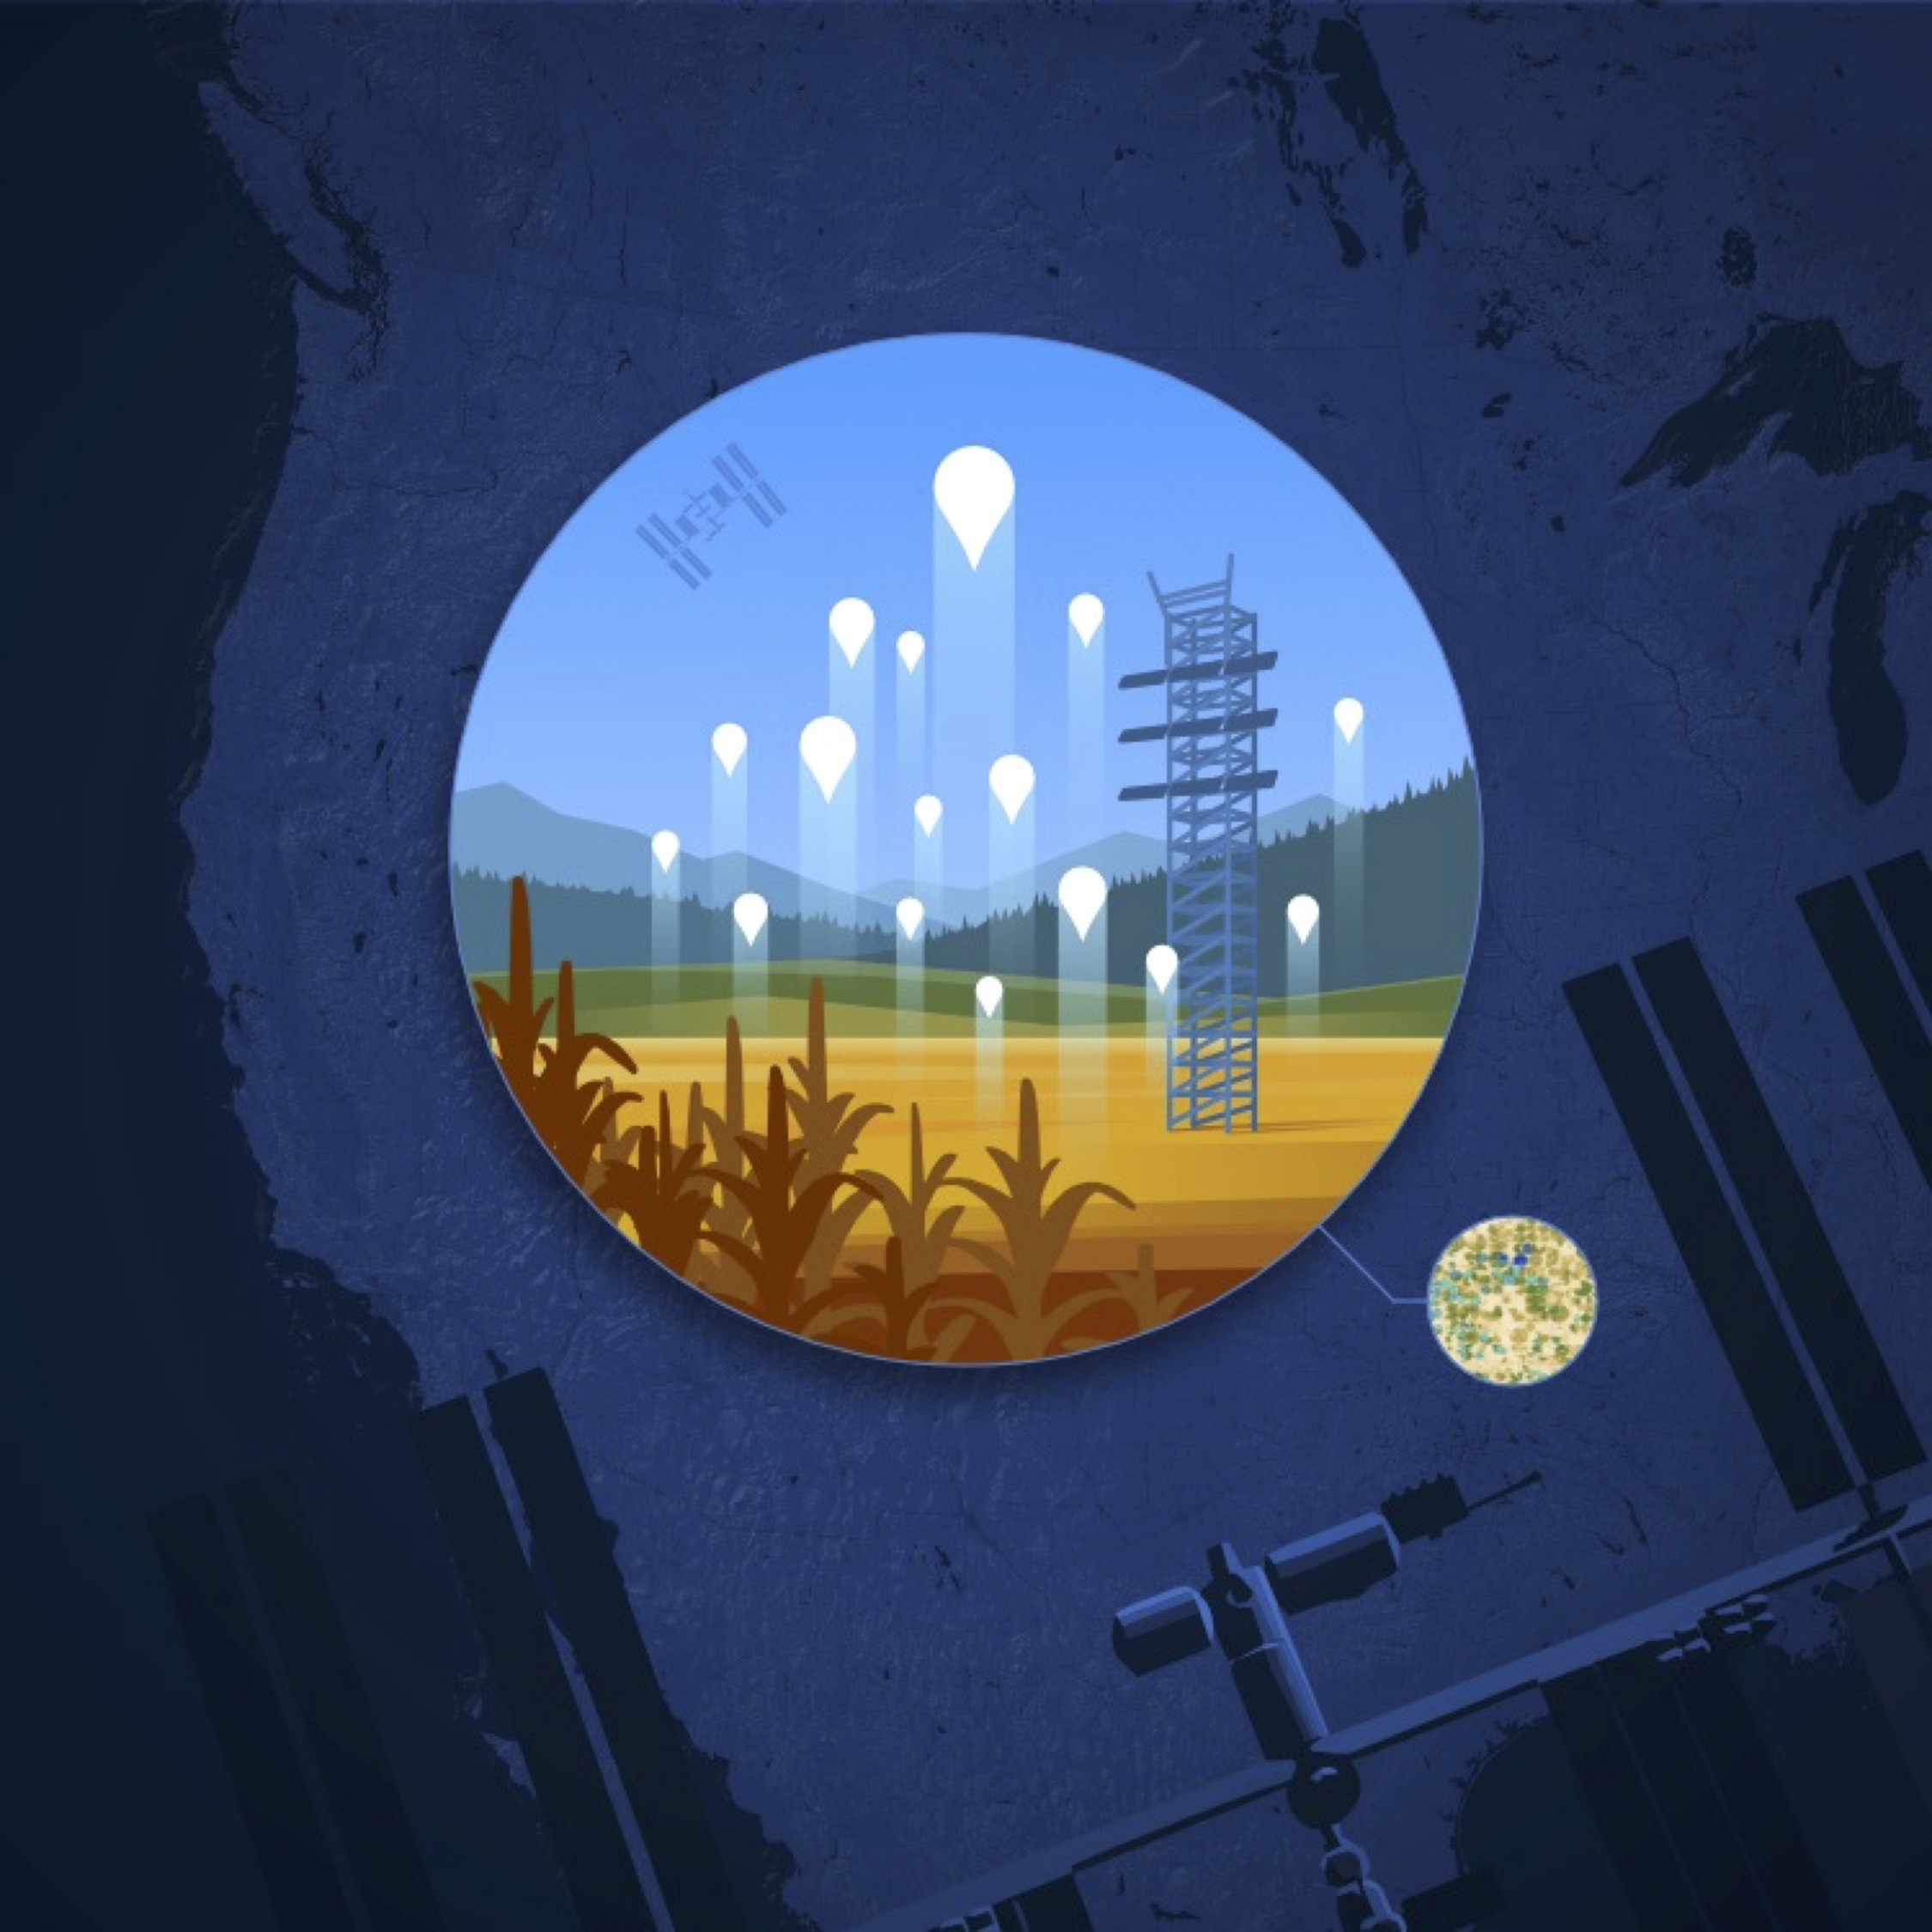
\includegraphics[scale=.03]{ECOSTRESS-BASE.jpg}};\end{tikzpicture}}
%%%%%%%%%%%%%%%%%%%%%%%%%%%%%%%%%%

\noindent\fbox{\begin{minipage}{.9665\textwidth}
			
	\vspace{1em}
	\begin{center}
		\textbf{\Large \underline{Motivation For Today's Tutorial: Drought \& Water Scarcity}}
	\end{center}
	
	\addcontentsline{toc}{section}{Motivation : Drought \& Water Scarcity}

	\vspace*{-1 em}
	
	\centerline{\includegraphics[width=.87\textwidth]{AmericasDrought.png}}

	The figure above was created for the United Nations report ``Drought in Numbers,'' calling for a global top priority commitment to drought preparedness and resilience across all regions. Drought is a complex crisis with roots not only in climate change, but also in social justice and public policy.

	\begin{itemize}
		\item More than 10 million people lost their lives due to major drought events in the past century, with over 90\% of these deaths occurring in developing countries (Guha-Sapir et al., 2021).
		\item By 2050, between 4.8 and 5.7 billion people will live in areas that are water-scarce for at least one month each year, up from 3.6 billion today (UN Water, 2021).
		\item \href{https://jeremydforsythe.github.io/icecream-tutorials/Tutorial11_ESI/GenderDrought.pdf}{Droughts can disproportionately affect women.} While the majority of rural farmers around the world are women, $<$15\% are the owners of agricultural lands, which means that the most affected women do not have the ability to make decisions about water scarcity and land use.
	\end{itemize}
	
\end{minipage}}

\section{Accessing ECOSTRESS ESI Data through A$\rho\rho$EEARS}

\subsection{ECOSTRESS Evaporative Stress Index (ESI) Data}

\vspace{.5em}

\centerline{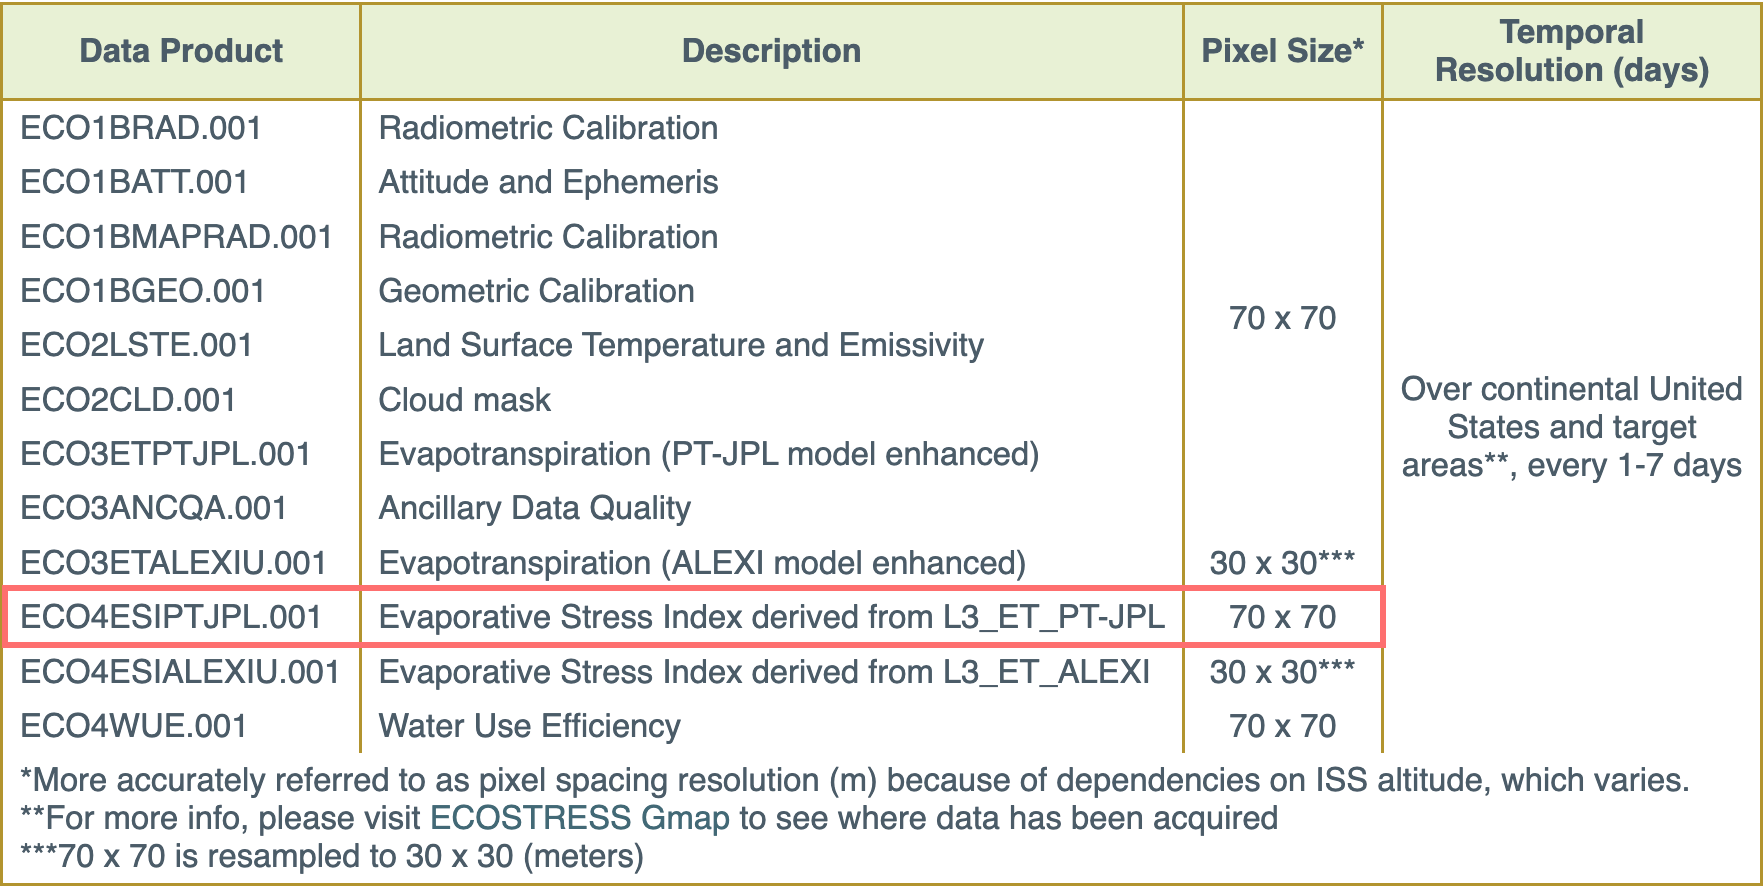
\includegraphics[width=.75\textwidth]{ECOSTRESS_DataProducts.png}}

\vspace{.5em}

In the previous tutorials, we learned that ECOSTRESS uses land surface temperatures to estimate evapotranspiration (ET). A related variable is the Evaporative Stress Index (ESI), which is a measure of potential drought conditions. It is a Level 4 (ECO4) ECOSTRESS data product that can be accessed through A$\rho\rho$EEARS:

\vspace{.5em}

\centerline{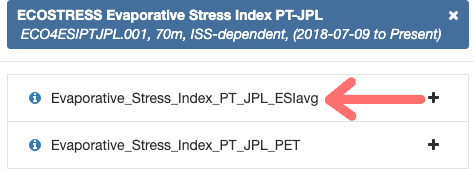
\includegraphics[width=.6\textwidth]{ESIecostress.png}}

\vspace{.5em}

For ECOSTRESS, the drought stress signal is derived from the ratio of actual evapotranspiration (AET) to potential evapotranspiration (PET):

\[
	ESI = \frac{AET}{PET}
\]

PET represents the theoretical maximum amount of ET that would occur in a location if unlimited water were available. ESI is a unitless metric (the numerator and denominator have the same units and they cancel out) that ranges from 0 to 1, with smaller proportions indicating higher water stress (minimal ET compared to PET) and higher proportions denoting no water stress (ET and PET are equal). 

\kulbox{\textbf{NOTE:} The range for ESI may be confusing, as a large number (nearing 1) indicates the absence of drought conditions, and a small number (nearing 0) suggests drought.}

\kulbox{\textbf{NOTE:} Confusingly, evaporative stress index can have different definitions from study to study. For example, the Mexico City map in the box below has a scale of -2.5 to 2.5, because it is estimated with a different formula. Keep an eye out for this!}

\begin{tcolorbox}[colback=yellow!5!white,colframe=IceCreamLeaf,title=\textbf{Today's Study Location : Mexico City}]
	\begin{multicols}{2}

	\centerline{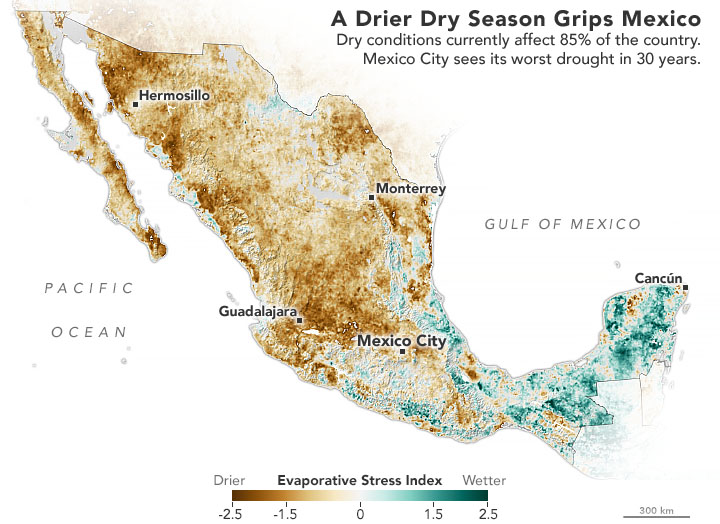
\includegraphics[width=\columnwidth]{mexico_esi_2021.png}}

	\columnbreak
		\begin{itemize}
			\item Most populous city in North America with $>$ 9.2 million people in the city center and $>$ 21.8 million people in the greater metropolitan area. 
			\item Northern Mexico's system of $>$ 60 reservoirs is currently $>$ 75\% drained, leading to water scarcity (the lack of available water for human use) for $>$ 30\% urban residents who do not have daily access to water.
		\end{itemize}
	\end{multicols}

	\begin{itemize}
		\item Mexico City sometimes has too little and sometimes too much water. In the dry season (October - April), droughts dry the land and deplete the water table. In the wet season (May - September), floods wash through its working-class neighborhoods.
		\item The year 2021 saw the worst drought conditions in more than three decades for Mexico City and brought predictions that 2022 might be worse. Today, we are using ECOSTRESS to compare the drought conditions of 2022 with the extreme conditions of 2021.
	\end{itemize}

\end{tcolorbox}

\subsection{Requesting Timeseries Point ESI Data in A$\rho\rho$EEARS}

So far, we have been using ECOSTRESS \textit{"Area"} data to create maps that visualize our variable of interest, but A$\rho\rho$EEARS also allows you to submit a \textit{"Point"} request. Instead of providing a shapefile or GeoJSON to define a set polygon area, we can provide GPS coordinates (latitude, longitude) to A$\rho\rho$EEARS, and it will return a timeseries of our variable of interest for the single pixel that encompasses our coordinates. Today, we are going to study ESI, but you can return this for any of the ECOSTRESS variables. 

1. To begin, go to \href{https://appeears.earthdatacloud.nasa.gov/}{https://appeears.earthdatacloud.nasa.gov/} and login with your credentials. 

2. Use the \textit{Extract} drop-down menu, but this time select \textit{Point}. Next, select \textit{Start a new request}. 

3. Enter a useful name for the request you are going to submit, maybe something like ``Mexico City ESI 2021-2022''. 

4. In the \textit{Uploaded coordinates (ID, Category, Lat, Long):} section enter the GPS coordinates for Mexico City as 19.42847, -99.12766.

5. Update the \textit{Start} and \textit{End} Date Fields for our dates of interest: 01/01/2021 to 12/31/2022.

\centerline{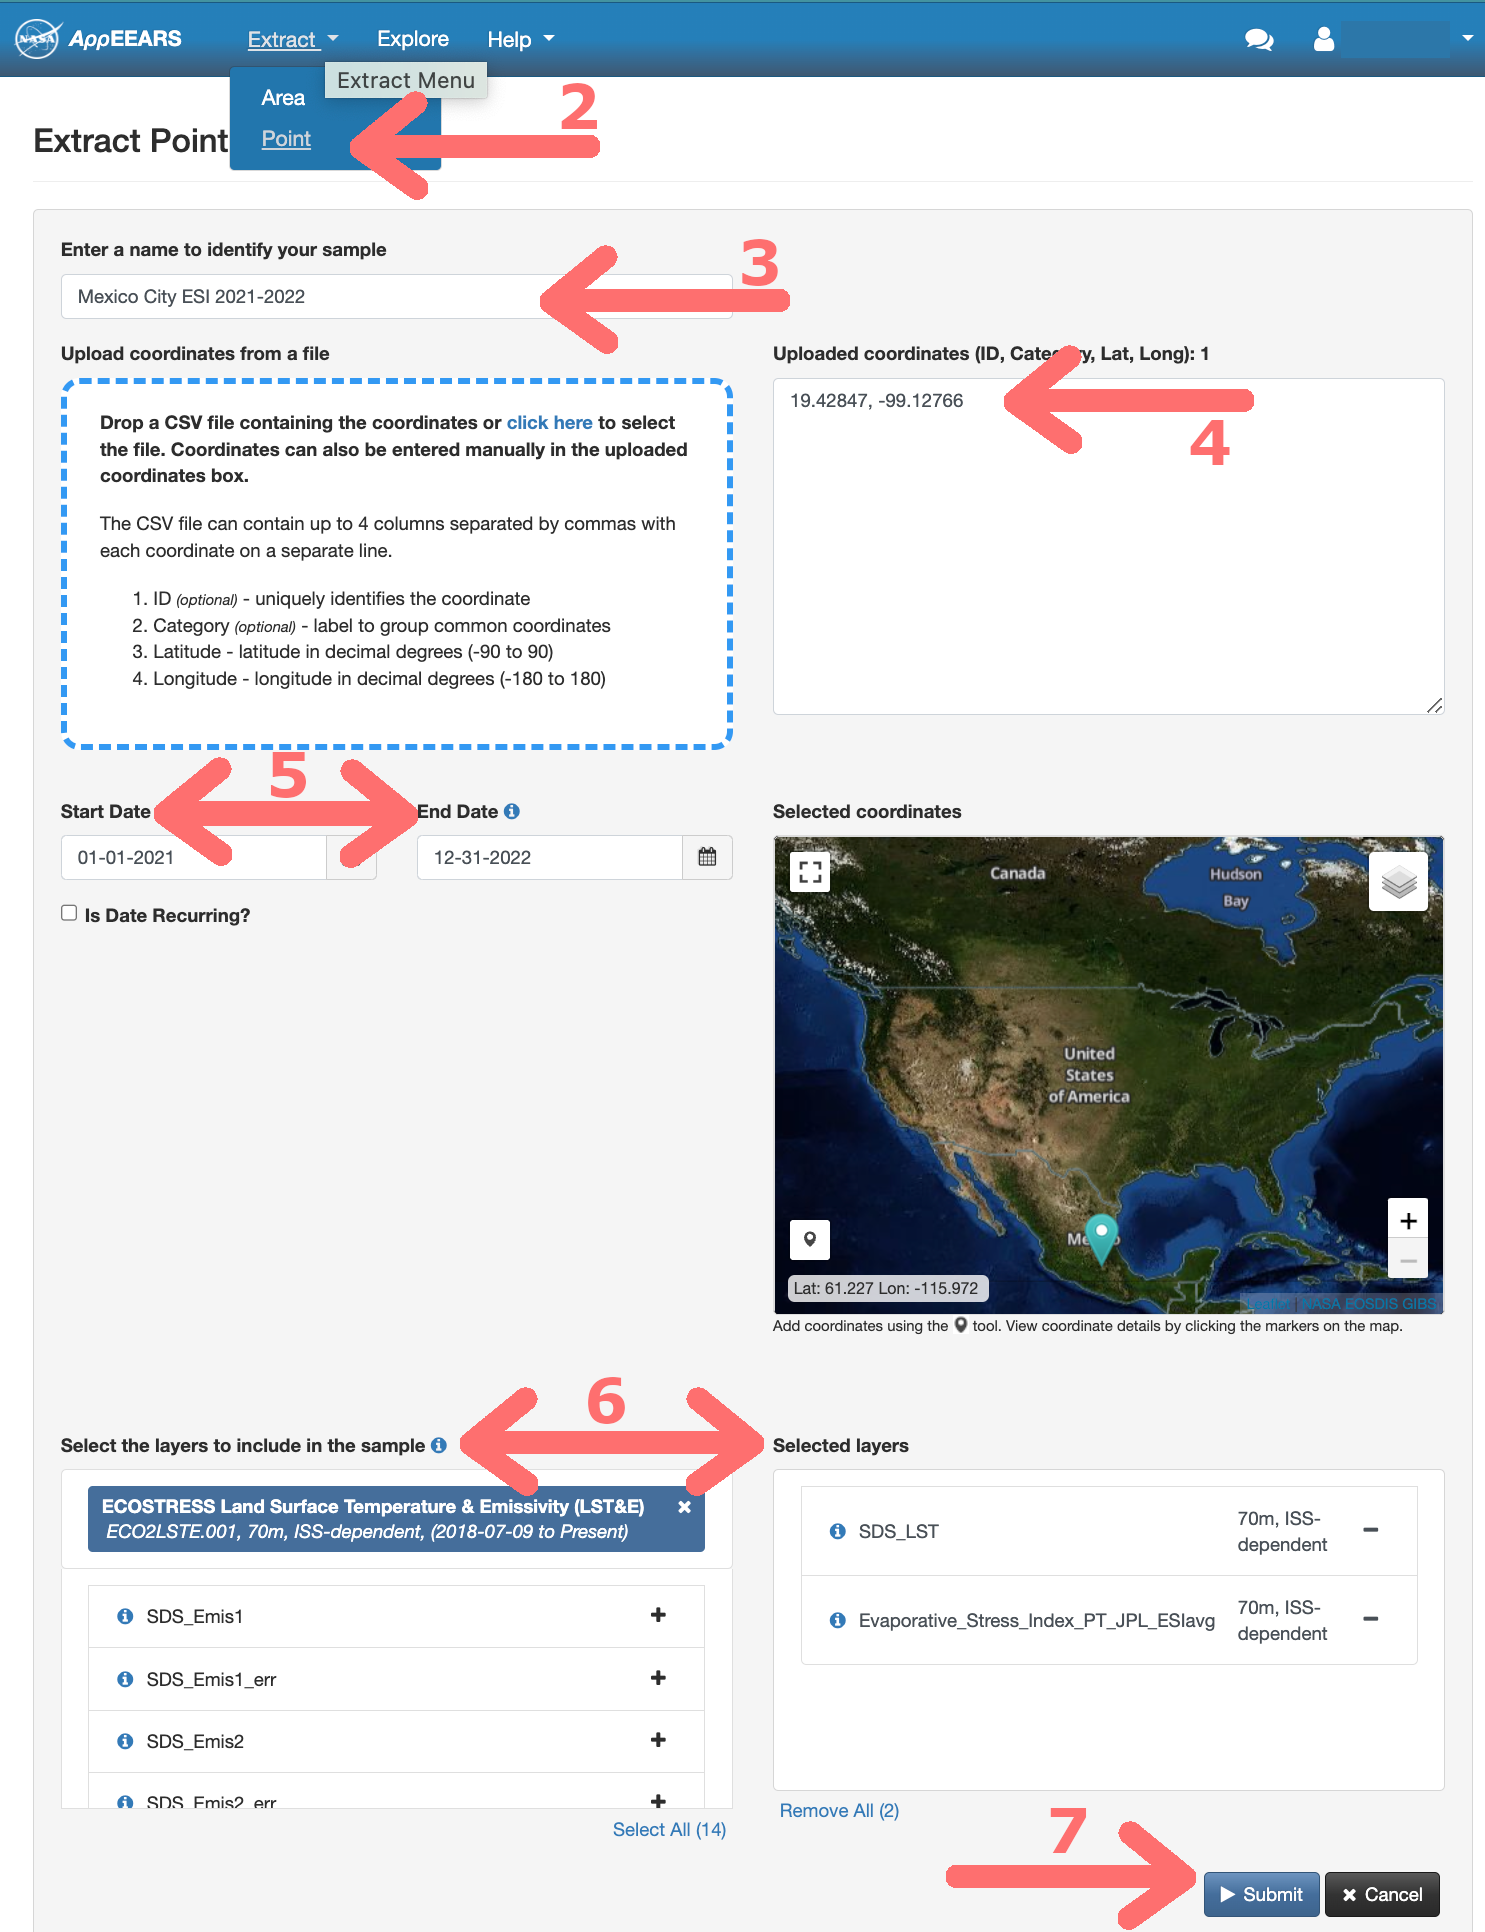
\includegraphics[width=.6\textwidth]{ESIpointRequest.png}}

\vspace{.5em}

6. Under \textit{Select the layers to include in the sample}, type the words ``ECOSTRESS'' and ``ESI'' Select \textit{ECOSTRESS Evaporative Stress Index PT-JPL}. Click on the ``+'' signs to add the following layers to your cart: 

\begin{itemize}
	\item Evaporative\textunderscore Stress\textunderscore Index\textunderscore PT\textunderscore JPL\textunderscore ESIavg
\end{itemize}

Next, clear the selection of the current category using the small ``x'' to the right of the \textit{ECOSTRESS Evaporative Stress Index PT-JPL} box.

\vspace{.5em}

Then, under \textit{Select the layers to include in the sample} type the words ``ECOSTRESS'' and ``LST,'' select \textit{ECOSTRESS Land Surface Temperature \& Emissivity (LST\&E)}. Click on the ``+'' signs to add the following layers to your cart: 

\begin{itemize}
	\item SDS\textunderscore LST
\end{itemize}

Clear the selection of the current category using the small ``x'' to the right of the \textit{ECOSTRESS Land Surface Temperature \& Emissivity (LST\&E)} box.

7. Click \textit{Submit} to complete the data request. At the top, you should see a green banner:

\vspace{.5em}

\centerline{
\includegraphics[width=\textwidth]{RequestSuccess.png}}

8. Use the \textit{Explore} drop-down at the top to monitor the status of your request. Point requests typically process faster than area requests because the system only needs to pull a single pixel from each scene.

\subsection{Requesting Area ESI Data in A$\rho\rho$EEARS}

While we wait for the point request, we are also going to create an area request so we can examine how the drought affects different parts of Mexico City. The procedure to download area ESI data through the A$\rho\rho$EEARS interface is the same as in previous tutorials on land surface temperature, evapotranspiration, and water use efficiency.

\subsubsection{Drawing and Exporting A GeoJSON File with QGIS}

9. First, we will begin by drawing an outline of the metropolitan region surrounding Mexico City and export it as a GeoJSON that we can load into A$\rho\rho$EEARS. 

\vspace{.5em}

\centerline{\includegraphics[width=\textwidth]{drawPolygonGeoJSON.png}}

\vspace{.5em}

10. Open QGIS and start a new project by selecting the \textit{Project} menu, then \textit{New}.

11. Then to add a basemap, find the \textit{HCMGIS} menu bar, select \textit{Basemap}, then pick your preferred map. Since we are outlining an urban area, we recommend using \textit{Google Satellite Hybrid}, which overlays streets and other Google maps data on satellite imagery. Note that clicking on a basemap type automatically adds a new layer to your map, as seen in the layer browser window.

12. Open the Lat Lon Tools window by selecting the \textit{Plugins} menu $\rightarrow$ \textit{Lat Lon Tools} $\rightarrow$ \textit{Zoom To Coordinate}.
	
13. Enter in the following GPS coordinates of Mexico City (formatted as latitude, longitude): 19.42847, -99.12766.
	
14. The \textit{Lat Lon Tools} plugin has found the GPS coordinates for Mexico City and marked them with a ``$+$'' on the map. 

15. Next, we want to draw a polygon (i.e., a line that forms the perimeter of the area of interest) that encompasses Mexico City, so that we can pull the request and download the data from A$\rho\rho$EEARS.
	
16. Zoom in to the GPS coordinates that we entered and marked with a ``$+$'' on the basemap using the \textit{zoom in} 
\includegraphics[height=\fontcharht\font`\B]{mActionZoomIn.png}, \textit{zoom out} 
\includegraphics[height=\fontcharht\font`\B]{mActionZoomOut.png}, and \textit{pan} 
\includegraphics[height=\fontcharht\font`\B]{mActionPan.png} buttons in the toolbar. If you are on a laptop, you could use the trackpad to do the same.

17. Next, we are going to create a new layer on the map by selecting the following menus: \textit{Layer} $\rightarrow$ \textit{Create Layer} $\rightarrow$ \textit{New Shapefile Layer...}

18. Select the ``...'' option next to the \textit{Filename} input window. Navigate somewhere you can remember (as always, we suggest creating a folder for each tutorial) and save it with a worthy filename. ``Mexico City Perimeter'' would be an appropriate name. 

19. Select \textit{UTF-8} for \textit{File encoding}.

20. Select \textit{Polygon} for geometry type. 

21. Leave the remaining options as their defaults and click \textit{OK}.

22. Now, it is time to draw the polygon. First, make sure that your new ``Mexico City Perimeter'' layer is highlighted in the \textit{Layers} window. 

23. Select the \textit{Toggle Editing} 
\includegraphics[height=\fontcharht\font`\B]{mActionToggleEditing.png} button on the toolbar to start editing the layer. 

24. Then select the \textit{Add Polygon Feature} 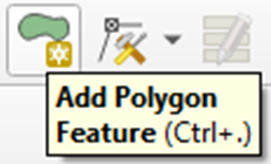
\includegraphics[height=10mm]{addpolygon.png} button to begin drawing. 

25. Draw a polygon that encompasses Mexico City. Don't worry too much about being perfect or strictly aligning to the city's borders; getting the basic shape is fine. Right-click on Windows or Linux and Ctrl-click on Mac to stop drawing when your shape is complete.

\kulbox{\textbf{NOTE:} Drawing a polygon in QGIS is both straightforward and nuanced. You use successive clicks with your mouse to create your desired shape. Simple forms such as squares or rectangles are easily achievable, whereas complex designs take some practice to master. It may take a couple of attempts to get it to look like what you are envisioning. You can always hit the ``ESC'' key to clear the polygon and start over.}

26. After you finish drawing, QGIS will prompt you for a feature ID. This is an arbitrary designation for our purposes today, so simply using the number 1 is my recommendation. 

27. Click \textit{OK}. 

28. Select the \textit{Toggle Editing} 
\includegraphics[height=\fontcharht\font`\B]{mActionToggleEditing.png} button from the toolbar to toggle off editing the layer. QGIS will prompt you to confirm saving the layer. Select \textit{Yes}.

29. To export your layer as a GeoJSON file: right-click (Windows or Linux) or ctrl-click (Mac) on the layer in your layer browser window. Then select \textit{Export}, then \textit{Save Feature As...}. In the next window make sure ``GeoJSON'' is the selected format.

\kulbox{\textbf{NOTE:} Make sure ``GeoJSON'' is the selected format. The default for QGIS is ``GeoPackage'', which isn't a format that A$\rho\rho$EEARS can read as an input. Also, there is a similar filetype ``GeoJSON Newline Delimited'' that A$\rho\rho$EEARS can also not read.}

30. Select the ``...'' option next to the \textit{Filename} input window to choose a logical location to save your GeoJSON file.

31. Name the file something appropriate, perhaps ``MexicoCity-Outline.'' 

32. Uncheck the box labeled ``Add saved file to map." 

33. Click ``OK''.

\subsubsection{Creating an Area Request for Mexico City in A$\rho\rho$EEARS}

Return to A$\rho\rho$EEARS to create a new area request. We have preselected dates with good data coverage (few-to-no clouds, orbit  that aligns with a single image for the area of interest) in 2021 \& 2022. 

34. Use the \textit{Extract} dropdown menu to select \textit{Area}. Next, select: \textit{Start a new request}. 

\vspace{.5em}

\centerline{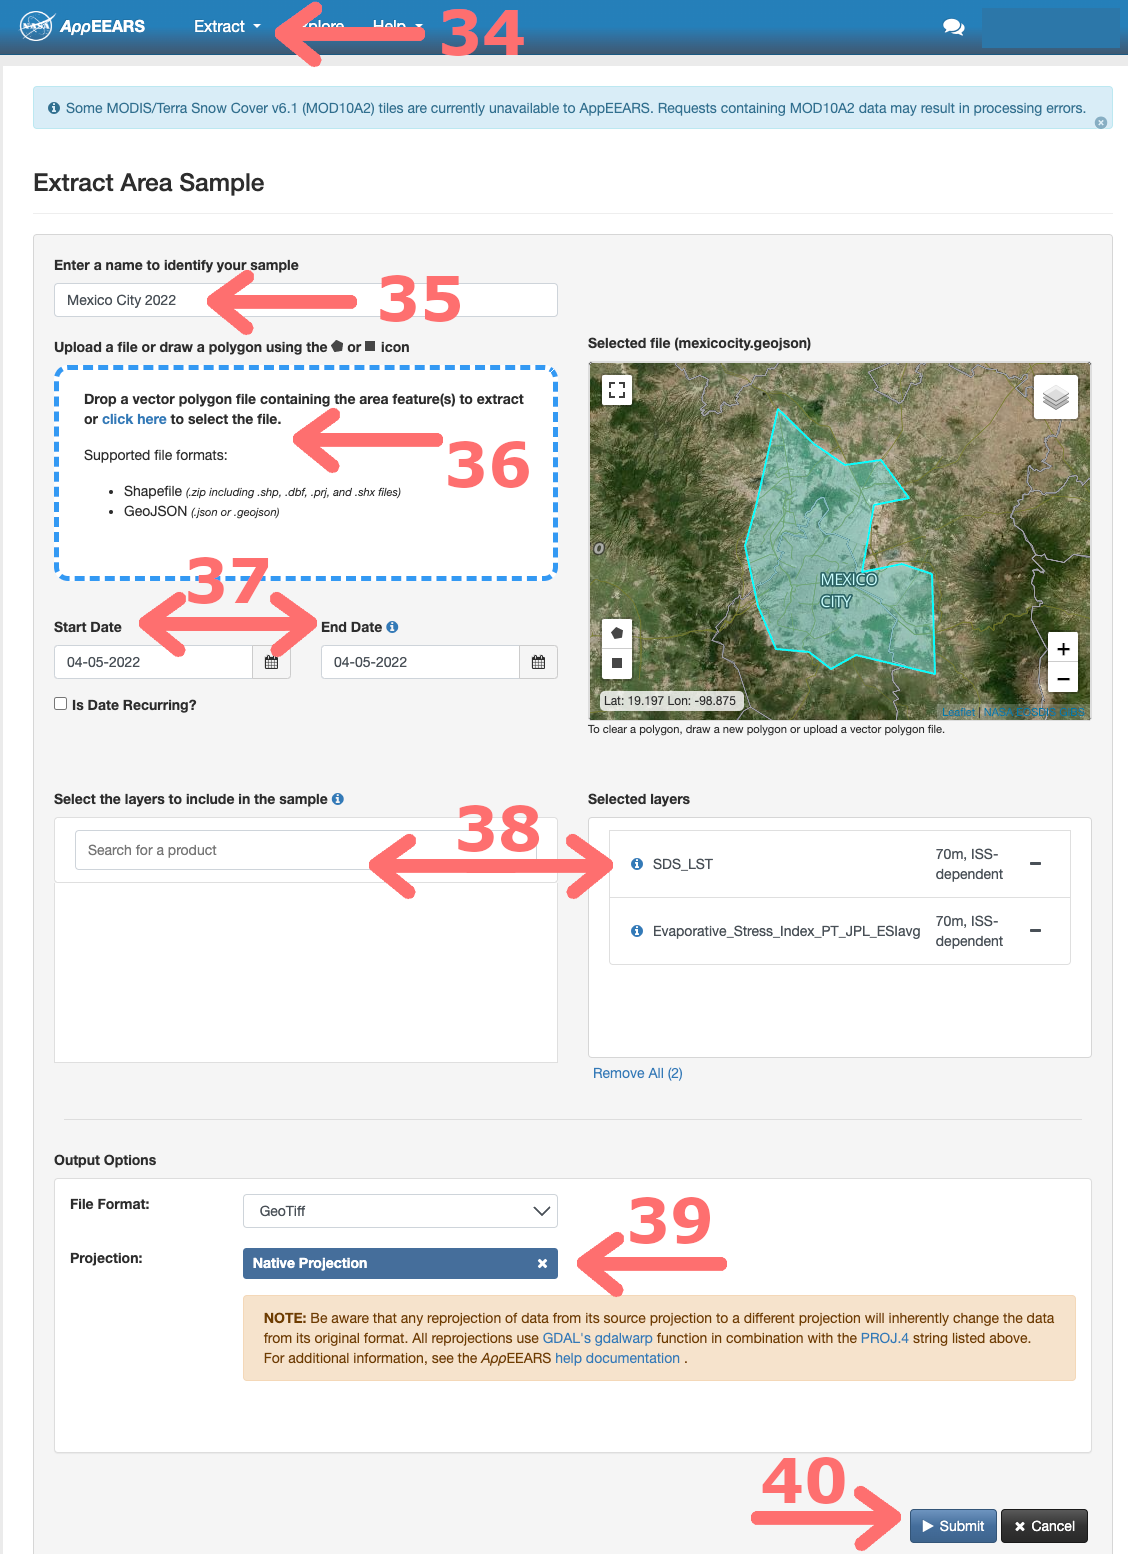
\includegraphics[width=.6\textwidth]{ESIareaRequest.png}}

\vspace{.5em}

35. Enter a useful name for the request you are going to submit, maybe something like ``Mexico City 2022''. 

36. Drag and drop (or use the \textit{click here to select the file} link) to upload the GeoJSON file we just exported in steps 10-33. The map should be updated with your polygon surrounding Mexico City.

37. Update the \textit{Start} and \textit{End} Date Fields for our preselected date of interest: 04/05/2022 to 04/05/2022.

38. Under \textit{Select the layers to include in the sample} type the words ``ECOSTRESS'' and ``ESI'' Select \textit{ECOSTRESS Evaporative Stress Index PT-JPL}. Click on the ``+'' signs to add the following layers to your cart: 

\begin{itemize}
	\item Evaporative\textunderscore Stress\textunderscore Index\textunderscore PT\textunderscore JPL\textunderscore ESIavg
\end{itemize}

Next, clear the selection of the current category using the small ``x'' to the right of the \textit{ECOSTRESS Evaporative Stress Index PT-JPL} box.

Then, under \textit{Select the layers to include in the sample} type the words ``ECOSTRESS'' and ``LST.'' Select \textit{ECOSTRESS Land Surface Temperature \& Emissivity (LST\&E)}. Click on the ``+'' signs to add the following layers to your cart: 

\begin{itemize}
	\item SDS\textunderscore LST
\end{itemize}

Clear the selection of the current category using the small ``x'' to the right of the \textit{ECOSTRESS Land Surface Temperature \& Emissivity (LST\&E)} box.

39. Under \textit{Output Options}, we want to use GeoTIFF (Geographic Tagged Image File Format; essentially, an image file where the corresponding geographic information is embedded in the file) and \textit{Native Projection} for projection.

40. Click \textit{Submit} to complete the data request. At the top, you should see a green banner:

\vspace{.5em}

\centerline{
\includegraphics[width=\textwidth]{RequestSuccess.png}}

\centerline{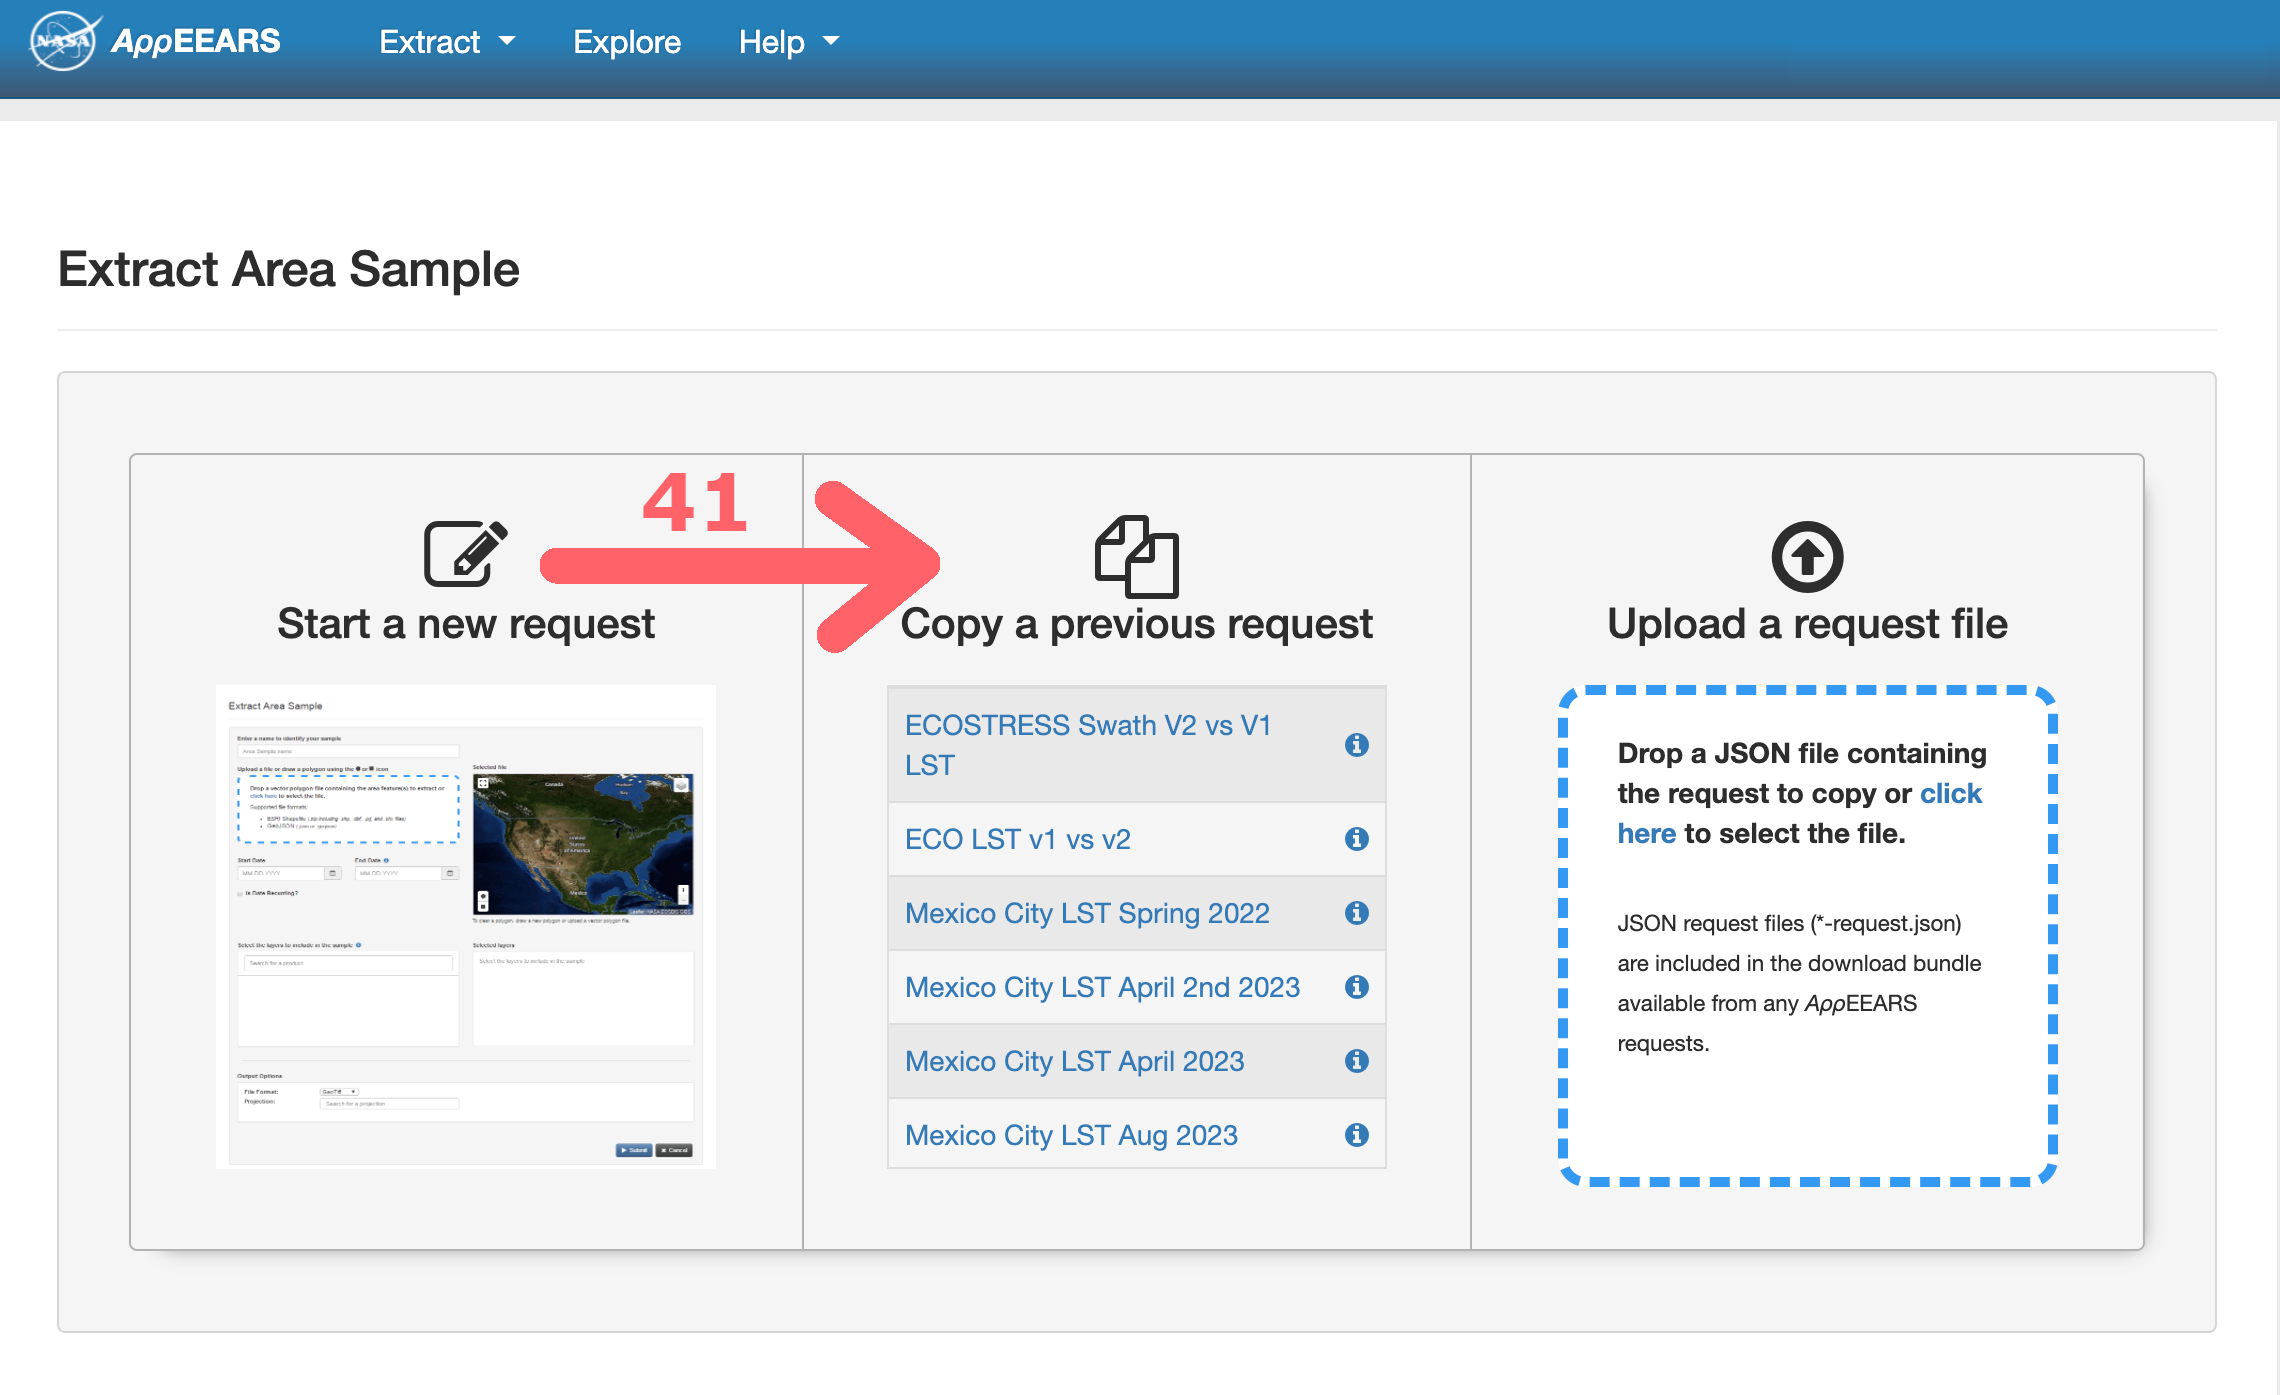
\includegraphics[width=\textwidth]{RepeatRequest.png}}

41. Repeat steps 34 - 40 with the same layers and GeoJSON file. Call the request ``Mexico City 2021'' and change the date to 4/28/2021. Or to be even more efficient from the \textit{Extract} page find your ``Mexico City 2022'' request in the ``Copy a previous request'' section and change the date to 4/28/2021.

42. Use the \textit{Explore} drop-down at the top to monitor the status of your request. Requests will likely go quickly, given that it is only one day's worth of data.

\section{Visualizing ESI Timeseries Point Data in A$\rho\rho$EEARS}

43. When your first timeseries point data request (``Mexico City ESI 2021-2022'') is complete, use the link on the \textit{Explore} page to access the details. A$\rho\rho$EEARS returns this data in a .csv spreadsheet that can be opened with free statistical software such as \href{https://www.r-project.org/about.html}{R}, the paid program Microsoft Excel, or the free alternative \href{https://www.libreoffice.org/}{Libreoffice Calc}. These software options can create graphs and run statistical comparisons. 

44. Additionally, you can use the A$\rho\rho$EEARS interface to do some light visualizations, which will serve our purposes today.

45. Our goal for the ESI timeseries point analysis is not to visualize the data in space, but rather to compare the differences between the two years (the known drought year of 2021 and 2022). The benefit of this point data is that A$\rho\rho$EEARS has conveniently packaged our variable of interest in an easy-to-manage format to track changes over time. The disadvantage of this type of data retrieval is that it can only be done for a single pixel per request. 

46. First, select the $Evaporative\textunderscore Stress\textunderscore Index\textunderscore PT\textunderscore JPL\textunderscore ESIavg$ layer.


The top panel displays the entire timeseries for the dates we have requested. The bottom panel compares years by plotting different years in our data in different colors. 

\vspace{.5em}

Notice that the dry season (October - April) has much higher drought stress (low ESI) compared to the wet season (May - September). Our goal was to compare 2022 to the known drought year of 2021. What conclusions can you draw from these data? 

\vspace{.5em}

\centerline{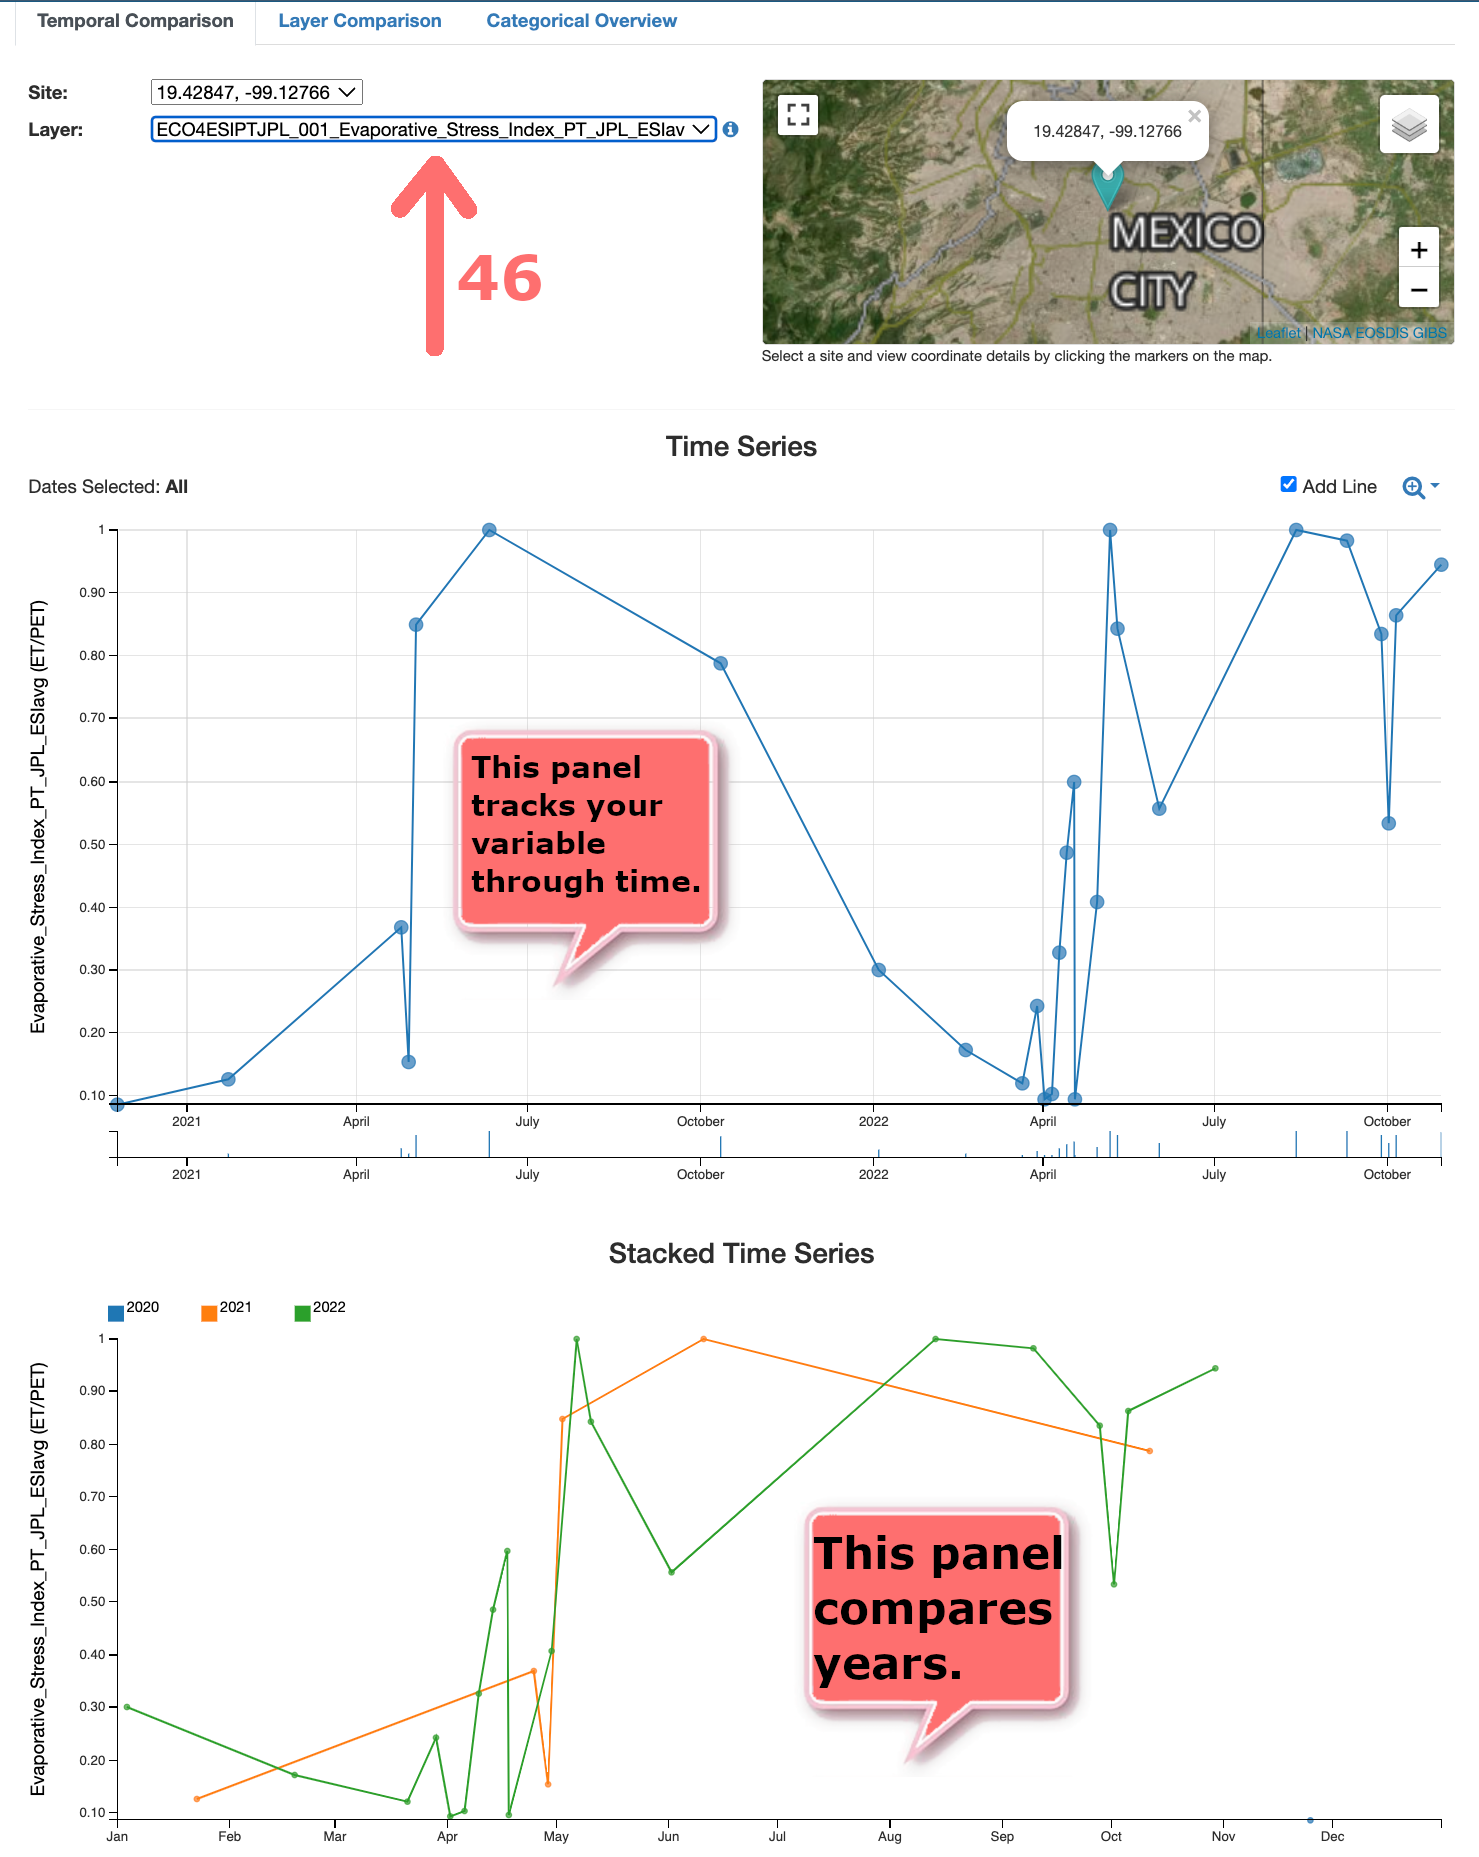
\includegraphics[width=.6\textwidth]{exploreESIpoint.png}}

\section{Visualizing Area ESI Data with QGIS}

\subsection{Download Area ESI Data in A$\rho\rho$EEARS}

\centerline{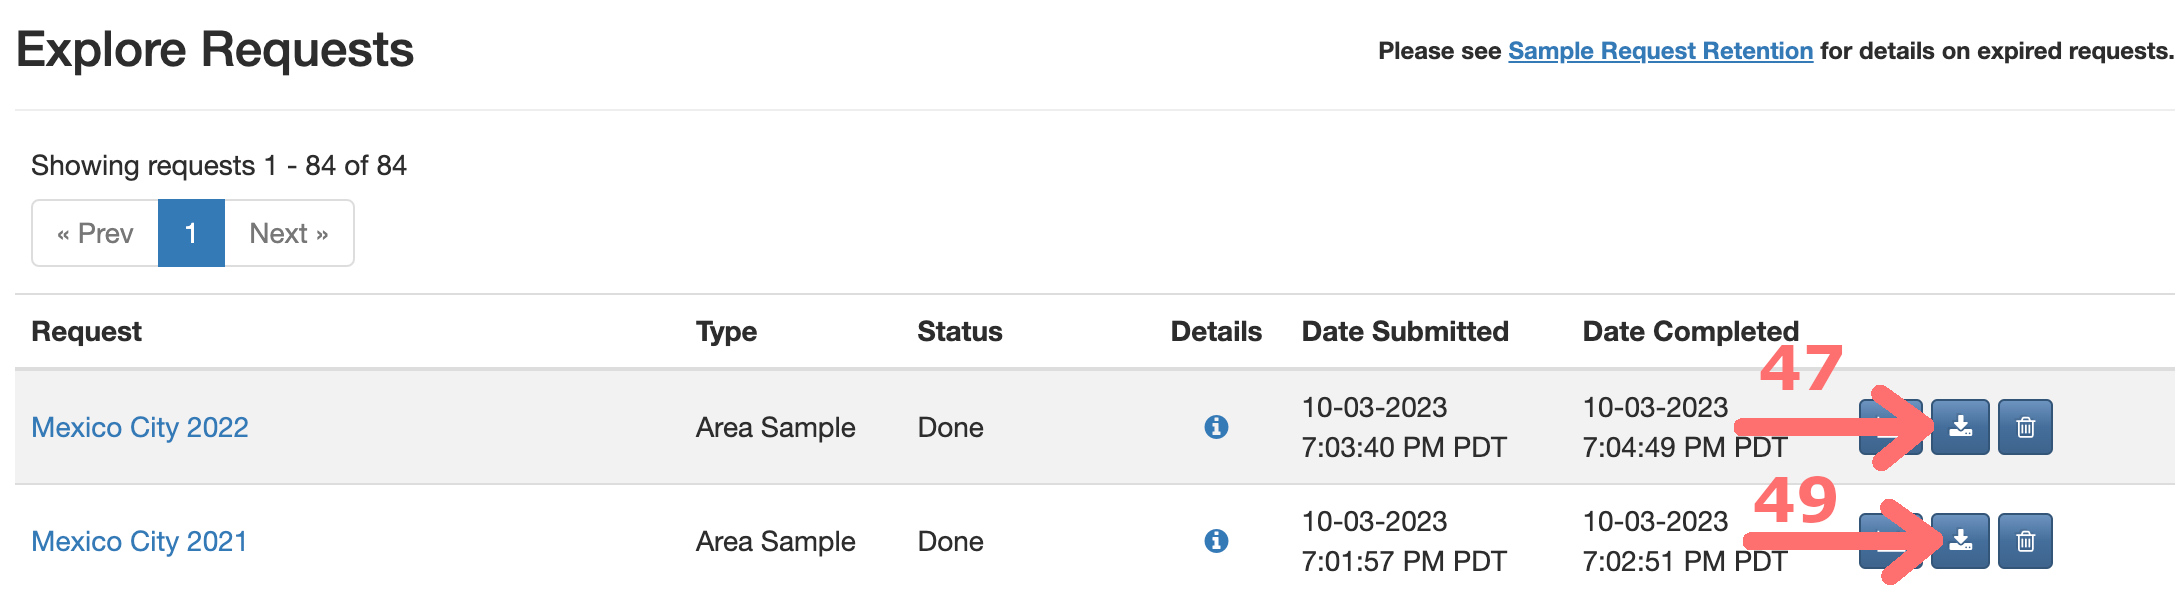
\includegraphics[width=.6\textwidth]{ESIareaRequestDown.png}}

\vspace{.5em}

47. By now, your area requests should be complete. From the \textit{Explore} dropdown menu at the top of the A$\rho\rho$EEARS interface, click the download button (middle blue button) for the first area request ``Mexico City 2022''. 

\vspace{.5em}

\centerline{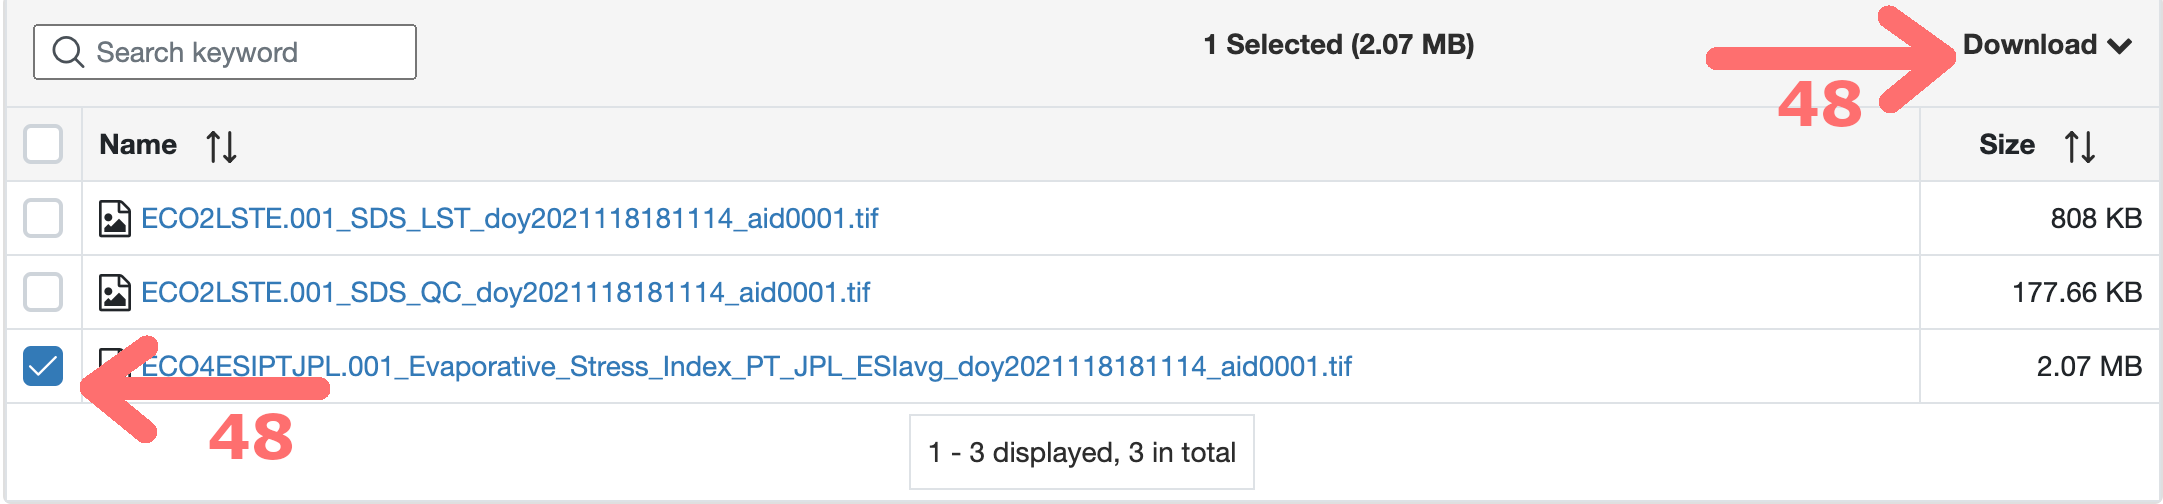
\includegraphics[width=.6\textwidth]{ESIareaDownload.png}}

\vspace{.5em}

48. Select the following filename: 

ECO4ESIPTJPL.001\textunderscore Evaporative\textunderscore Stress\textunderscore Index\textunderscore PT\textunderscore JPL\textunderscore ESIavg\textunderscore doy2022095170707\textunderscore aid0001.tif. Download the file using the \textit{Download} button, which for some reason does not look much like a button, in the upper right corner of the screen. Save the file somewhere you can remember. 

49. Repeat steps 47 - 48 to download the file from the second request ``Mexico City 2021'' to download the following filename: 

ECO4ESIPTJPL.001\textunderscore Evaporative\textunderscore Stress\textunderscore Index\textunderscore PT\textunderscore JPL\textunderscore ESIavg\textunderscore doy2021118181114\textunderscore aid0001.tif 

\subsection{Adding a Google Satellite Basemap}

50. Switch to QGIS and start a new project by selecting the \textit{Project} menu, then \textit{New}.

51. To add a basemap, find the \textit{HCMGIS} menu bar, select \textit{Basemap}, then pick your preferred map. For today's map, we will use \textit{Google Satellite}. Note that clicking on a basemap type automatically adds a new layer to your map, as seen in the layer browser window.

\vspace{.5em}

\centerline{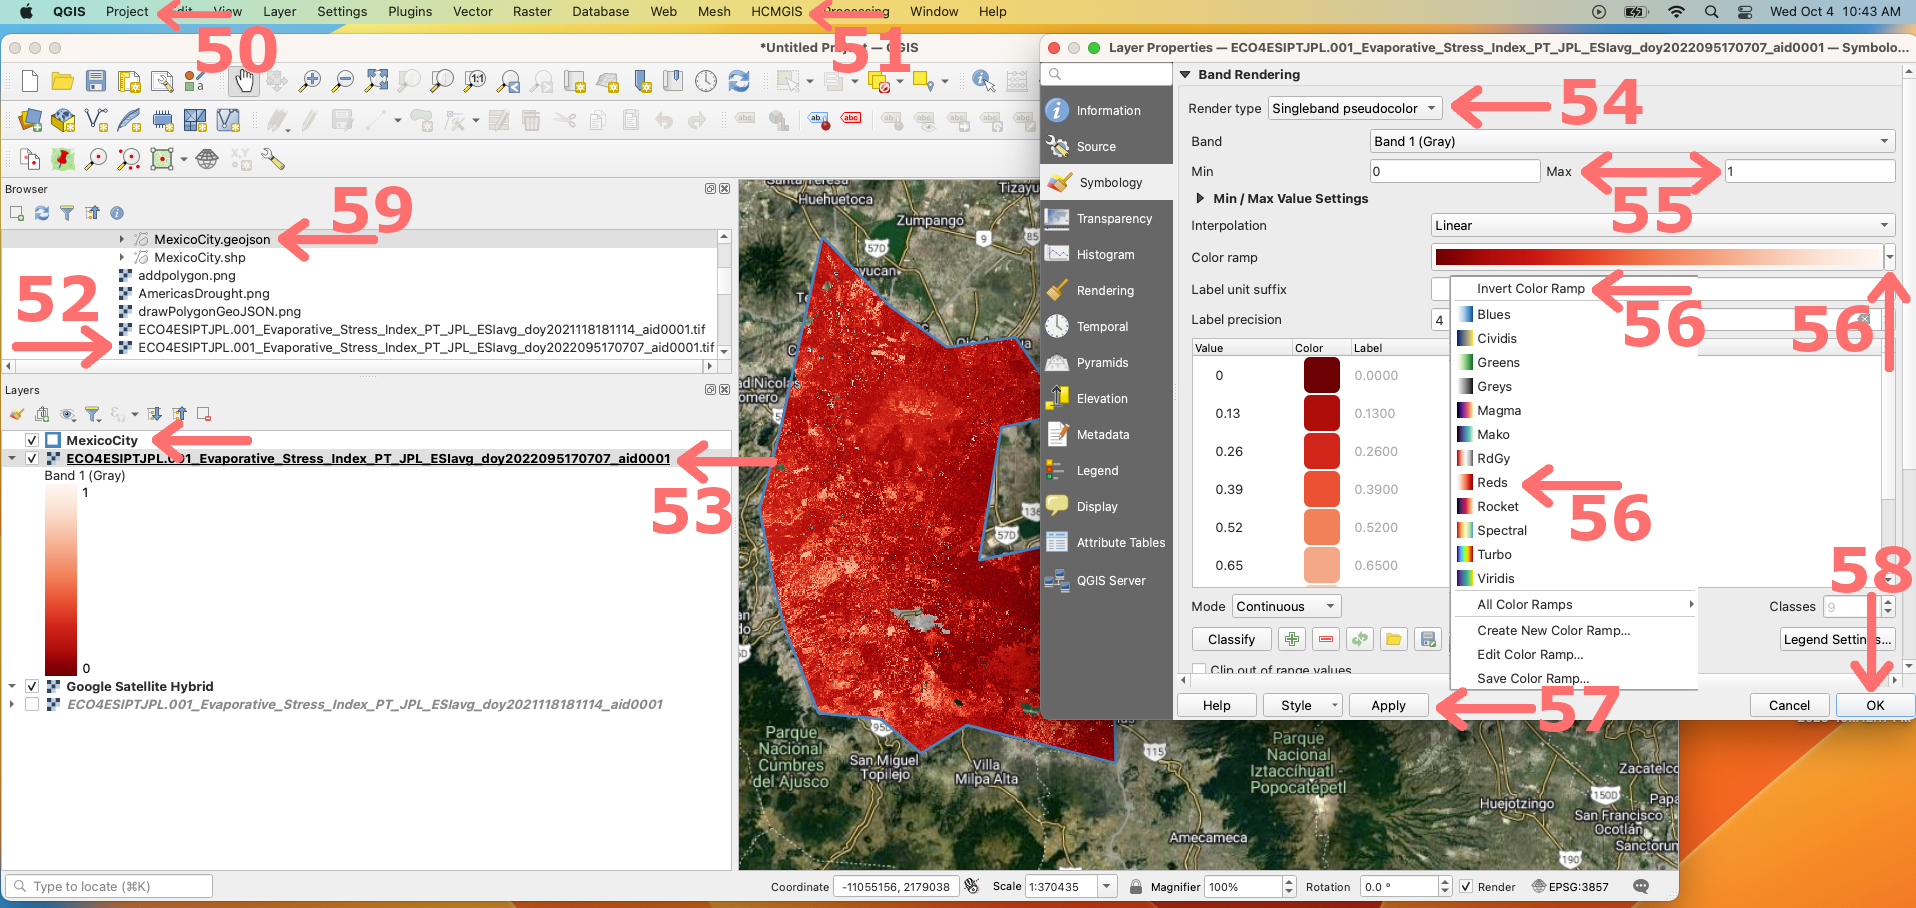
\includegraphics[width=\textwidth]{addESIlayer.png}}

\subsection{Add in ESI layer}

52. Use the \textit{browser} window to find the folder where you saved the 2022 ESI file: \\ ECO4ESIPTJPL.001\textunderscore Evaporative\textunderscore Stress\textunderscore Index\textunderscore PT\textunderscore JPL\textunderscore ESIavg\textunderscore doy2022095170707\textunderscore aid0001.tif. Double-click on it to add it to your map. Again, notice that the layer from this GeoTIFF file is now also listed in the \textit{Layers} window.

\kulbox{\textbf{NOTE:} QGIS can automatically zoom to your layer's area of interest by right clicking (ctrl-click on Mac) on the layer and selecting \textit{Zoom to Layer(s).}}

53. Now, you have ECOSTRESS ESI data on your map, but we need to change it from grayscale. Right-click (ctrl-click on Mac) on the layer name in the \textit{Layers} window and select \textit{Layer Properties}. 

54. On the menu bar to the left, select \textit{Symbology} and change \textit{Render type} to Singleband pseudocolor. 

55. QGIS has automatically determined the minimum and maximum values from the datafiles; however, we are going to want to compare two different years and need to match them. The ESI range is 0-1, so specify 0 as the minimum and 1 as the maximum. 

56. Now, we need to change the color ramp to effectively communicate ESI. Let's select the ``Reds'' option, but remember that the scale for ESI is inverted (0 indicating drought stress \& 1 indicating non drought conditions). To address this, check the \textit{invert color ramp} checkbox. 

57. Click \textit{apply}.

58. Then click \textit{ok}.

59. Finally, add the polygon border from your Mexico City GeoJSON file by double clicking on it in the \textit{Browser} window. Right-click (ctrl-click on Mac) on the layer in the \textit{Layers} window and change the symbology to \textit{outline blue}. 

60. Repeat steps 52 - 59 for the Mexico City 2021 data to create two separate maps comparing. How does 2022 compare to the 2021 year of extreme drought in Mexico City? What conclusions can you draw from the ECOSTRESS observations of ESI?

\begin{tcolorbox}[colback=yellow!5!white,colframe=MACred,title= \vspace{.2em} \Large Make a Map Assignments]
	\addcontentsline{toc}{section}{Make a Map Assignments}
	\large
	\begin{enumerate}
		\item Make a map of evaporative stress index for an area of interest. Try to identify an interesting comparison or contrast based on some aspect of climate, edaphic (soil) conditions, plant community composition or structure, land use, or some disturbance. If you complete your map and do not find strong differences, don’t worry! The most important part of this exercise is to practice asking a question, collecting the data to answer your question, and thinking about what you found. 
        \item Find a classmate and compare maps. Is your classmate doing anything differently that can help improve your map? If so, revise accordingly! 
        \item Submit your evaporative stress index map, along with a short description. In particular, your description might address any interesting observations and address any limitations of your analysis.
	\end{enumerate}
\end{tcolorbox}

\begin{tcolorbox}[colback=yellow!5!white,title=\textbf{Datafiles}]
	\addcontentsline{toc}{section}{Datafiles}
	\large
	In case you encountered any issues with the A$\rho\rho$EEARS database, here are copies of the ECOSTRESS GeoTIFF file for Mexico City ESI:
	\begin{itemize}
		\item 2022: \href{https://jeremydforsythe.github.io/icecream-tutorials/Tutorial10_ESI/ECO4ESIPTJPL.001_Evaporative_Stress_Index_PT_JPL_ESIavg_doy2022095170707_aid0001.tif}{\small ECO4ESIPTJPL.001\textunderscore Evaporative\textunderscore Stress\textunderscore Index\textunderscore PT\textunderscore JPL\textunderscore ESIavg\textunderscore doy2022095170707\textunderscore aid0001.tif}
            \item 2021: \href{https://jeremydforsythe.github.io/icecream-tutorials/Tutorial10_ESI/ECO4ESIPTJPL.001_Evaporative_Stress_Index_PT_JPL_ESIavg_doy2021118181114_aid0001.tif}{\small ECO4ESIPTJPL.001\textunderscore Evaporative\textunderscore Stress\textunderscore Index\textunderscore PT\textunderscore JPL\textunderscore ESIavg\textunderscore doy2021118181114\textunderscore aid0001.tif}
	\end{itemize}
\end{tcolorbox}

%%%%%%%%%%%%%%%%%%%%%%%%%%%%%%%%%%%%%%%%%%%%%%%%%%%%%%%%%%%%%%%%%%%%%%%%%%%%%%%%%%% End of Document
\vfill

\hrule

\vspace{1em}

\small \textbf{Recommended Citation:} Forsythe, J.D., G.R. Goldsmith, and J.B. Fisher. 2023. Observing Earth from Above Tutorials. Chapman University. \url{https://jeremydforsythe.github.io/icecream-tutorials/}

\vspace{1em}

This work is supported by funding from NASA ECOSTRESS Mission Grant \#80NSSC23K0309 (I.C.E. C.R.E.A.M.: Integrating Communication of ECOSTRESS Into Community Research, Education, Applications, and Media) and is openly licensed via \href{https://creativecommons.org/licenses/by-nc/4.0/}{CC BY-NC}.

\end{document}
